\section{Versuchsaufbau}
\label{sec:Versuchaufbau}

Der verwendete Versuchsaufbau nutzt als Photonenquelle eine Spektrallampe (siehe Abbildung \ref{fig:Versuchsaufbau}). Das Licht wird, um schlussendlich nur $D_1$-Licht zu erhalten, durch eine Sammellinse fokussiert, daraufhin die entsprechende Wellenlänger heraus gefiltert und linear polarisiert. Mit einem $\lambda /4$-Plättchen wird eine Phasenverschiebung von $\pi /2$ erzeugt, wodruch das Licht rechtszirkular polarisiert wird. Das Licht trifft dann auf eine Dampfzelle in der sich das $\ce{^{87}_{}Rb}$ und $\ce{^{85}_{}Rb}$-Gas befindet. Um diese Zelle herum befinden sich drei Helmholtz-Spule und eine Sweep-Spule, die die benötigte Hochfrequenz erzeugt. Danach wird das Licht auf eine Si-Doide fokussiert, die die Intensität bestimmt und auf einem angeschlossen  Oszilloskop dargestellt.

\begin{figure}
	\centering
	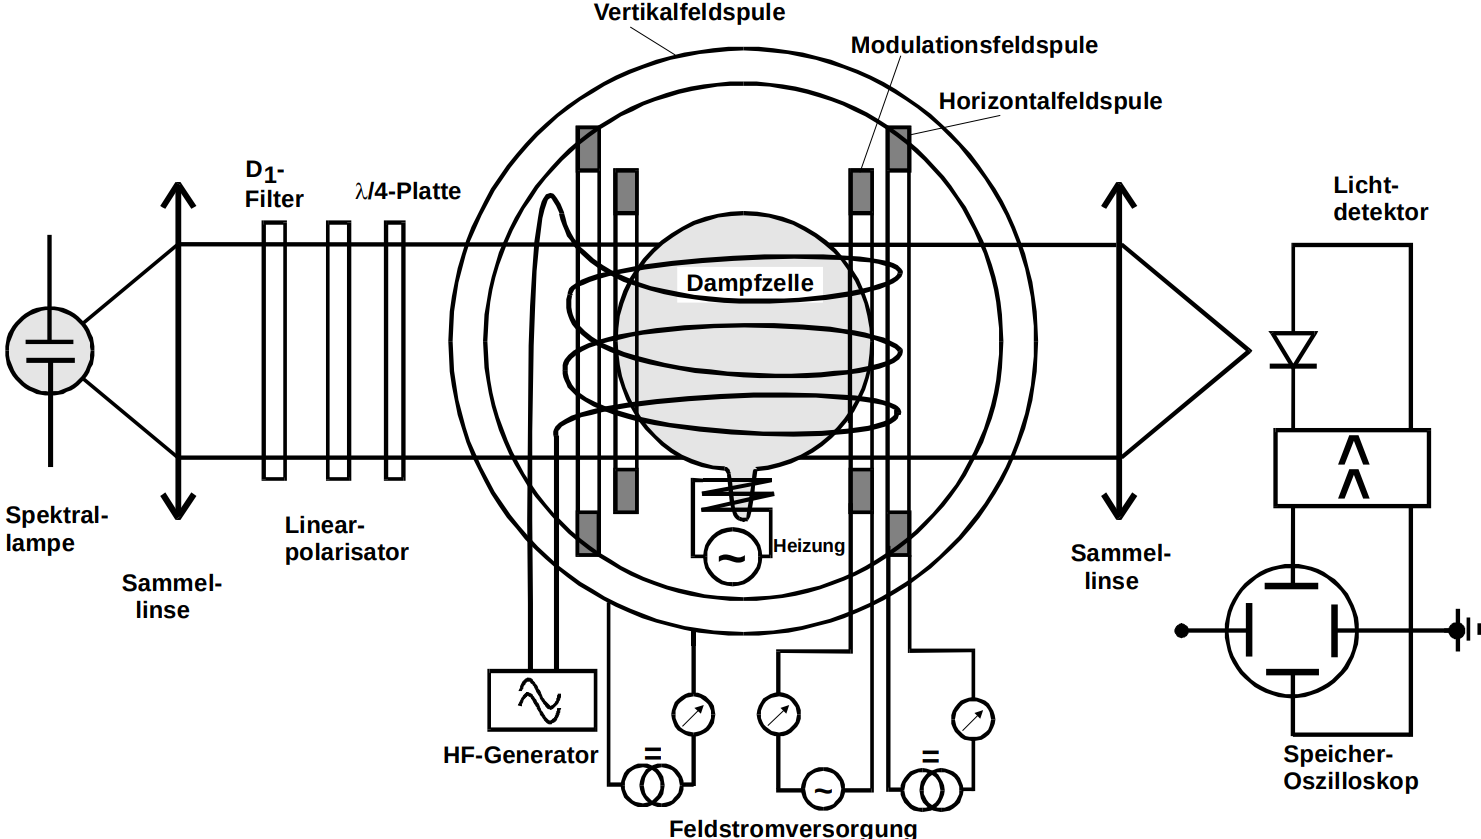
\includegraphics[width=0.8\textwidth]{ressources/Aufbau.png}
	\caption{Versuchsaufbau. \cite{skript}}
	\label{fig:Versuchsaufbau}
\end{figure}